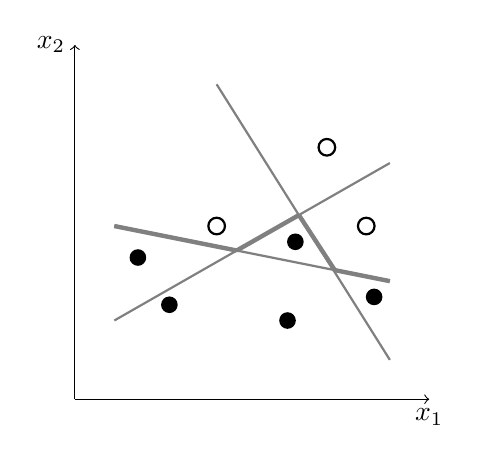
\begin{tikzpicture}[scale=1]
  % osi
  \draw[->] (0,0) -- (4.5,0) node[below] {$x_1$};
  \draw[->] (0,0) -- (0,4.5) node[left] {$x_2$};

  % trieda 1 - štvorčeky
  \foreach \x/\y in {1.8/2.2, 3.7/2.2, 3.2/3.2}
    \draw[thick] (\x,\y) circle (3 pt);

  % trieda 2 - plné štvorce
  \foreach \x/\y in {1.2/1.2, 0.8/1.8, 2.7/1.0, 2.8/2.0, 3.8/1.3}
    \fill (\x,\y) circle (3 pt);

  % rozhodovacie hranice
  \draw[gray, thick] (0.5,2.2) -- (4.0,1.5);
  \draw[gray, thick] (0.5,1.0) -- (4.0,3.0);
  \draw[gray, thick] (4.0,0.5) -- (1.8,4.0);

  % zvýraznená rozhodovacia hranica výstupného neurónu
  % zvýraznená rozhodovacia hranica výstupného neurónu
\draw[ultra thick, gray] (0.5,2.2) -- (2.055,1.889); % L2
\draw[ultra thick, gray] (2.055,1.889) -- (2.845,2.339); % L3
\draw[ultra thick, gray] (2.845,2.339) -- (3.3,1.64);    % L3 (ďalší úsek)
\draw[ultra thick, gray] (3.3,1.64) -- (4.0,1.5);    % L1 alebo L2 (podľa kontextu)

\end{tikzpicture}